\subsection{Monitoraggio e Intervento}
L'utilizzo della suite \textbf{Ipopt} e' stato fatto per l'applicazione di un sistema
di monitoraggio e intervento all'interno del modello di simulazione. Successivamente l'idea
di utilizzare un integrazione con la suite \textbf{SciML.ai} verra' sfruttata per 
aggiungere algoritmi di Machine Learning per rendere piu' realistico e consistente il modello 
nelle sue predizioni e scelte.

\subsubsection{Controllore con Ipopt}

\begin{minipage}{\linewidth}
	\centering
	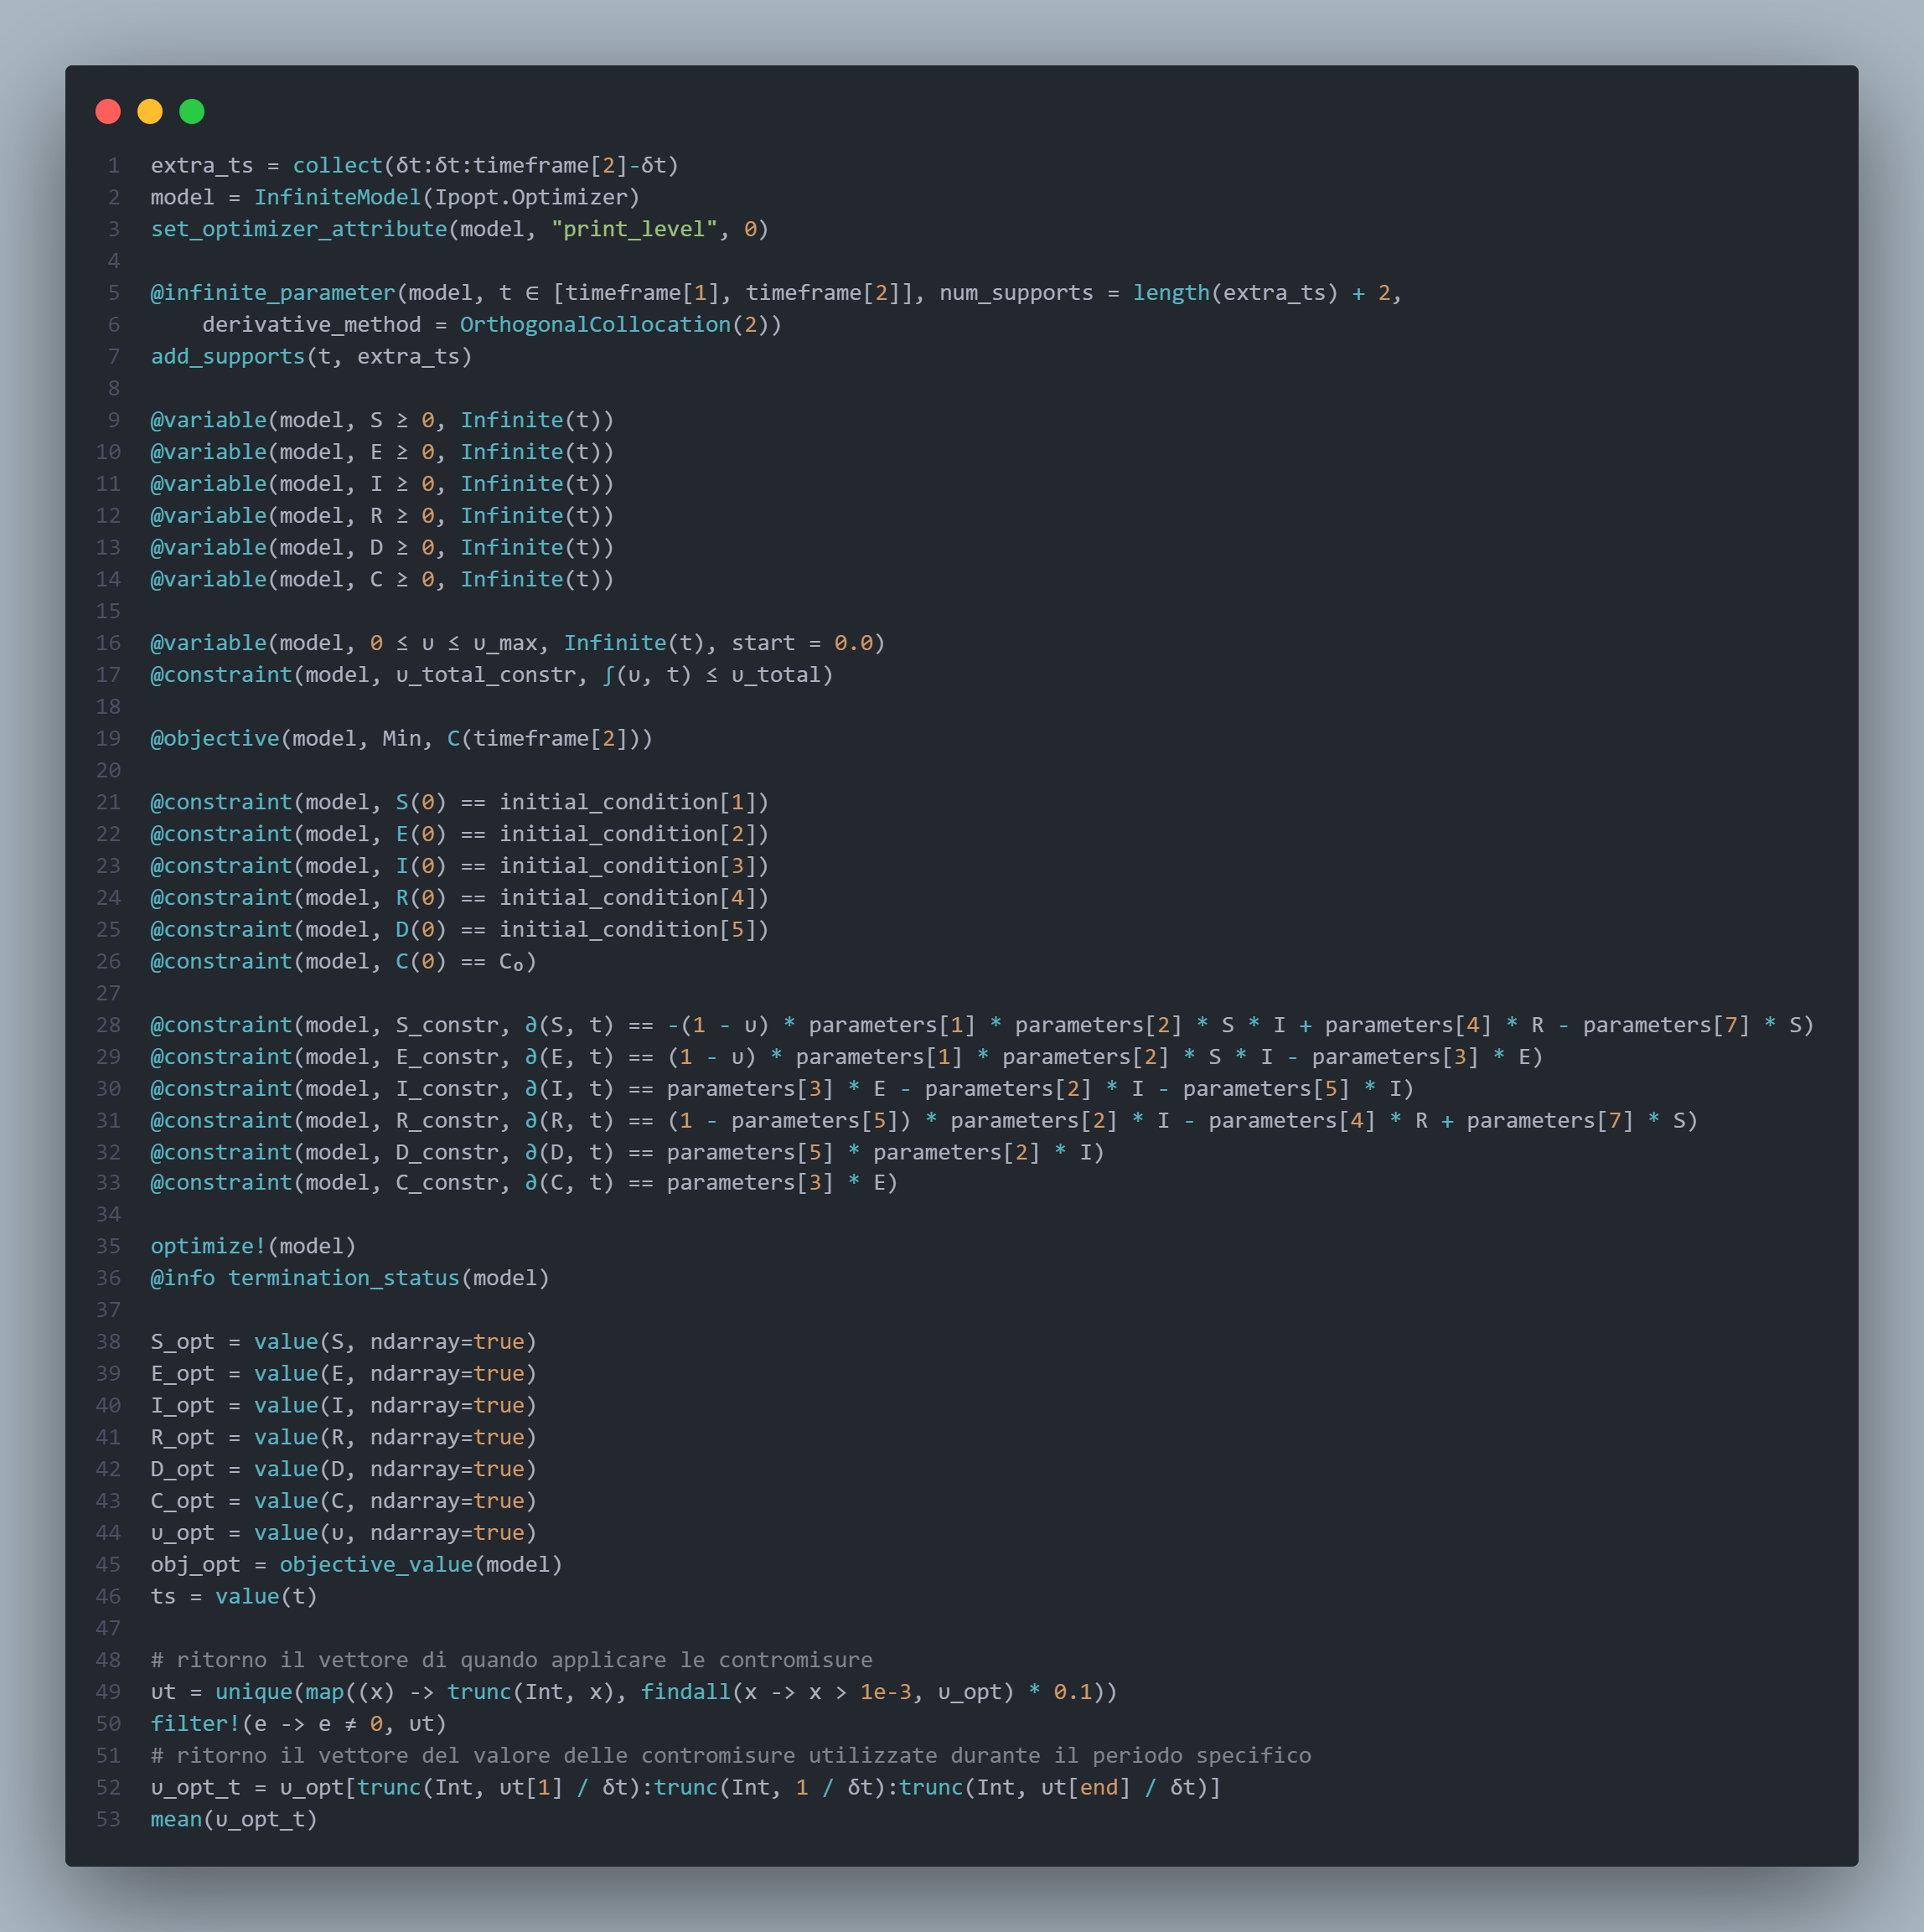
\includegraphics[width=\textwidth]{img/controller_ipopt.png}
	\captionof{figure}{Definizione del controllore tramite Ipopt}
	\label{fig:controller_ipopt}
\end{minipage}

L'approccio generale e' stato semplice ma efficace, in quanto viene definito un modello 
per raccogliere tutte le informazioni relative e necessarie per l'algoritmo di ottimizzazione
e successivamente vengono definite le regole che governano il comportamento del modello. 

Le regole in questione sono principalmente le stesse che sono usate per descrivere il modello SEIR
che viene utilizzato all'interno del modello ad agente.

\begin{minipage}{\linewidth}
	\centering
	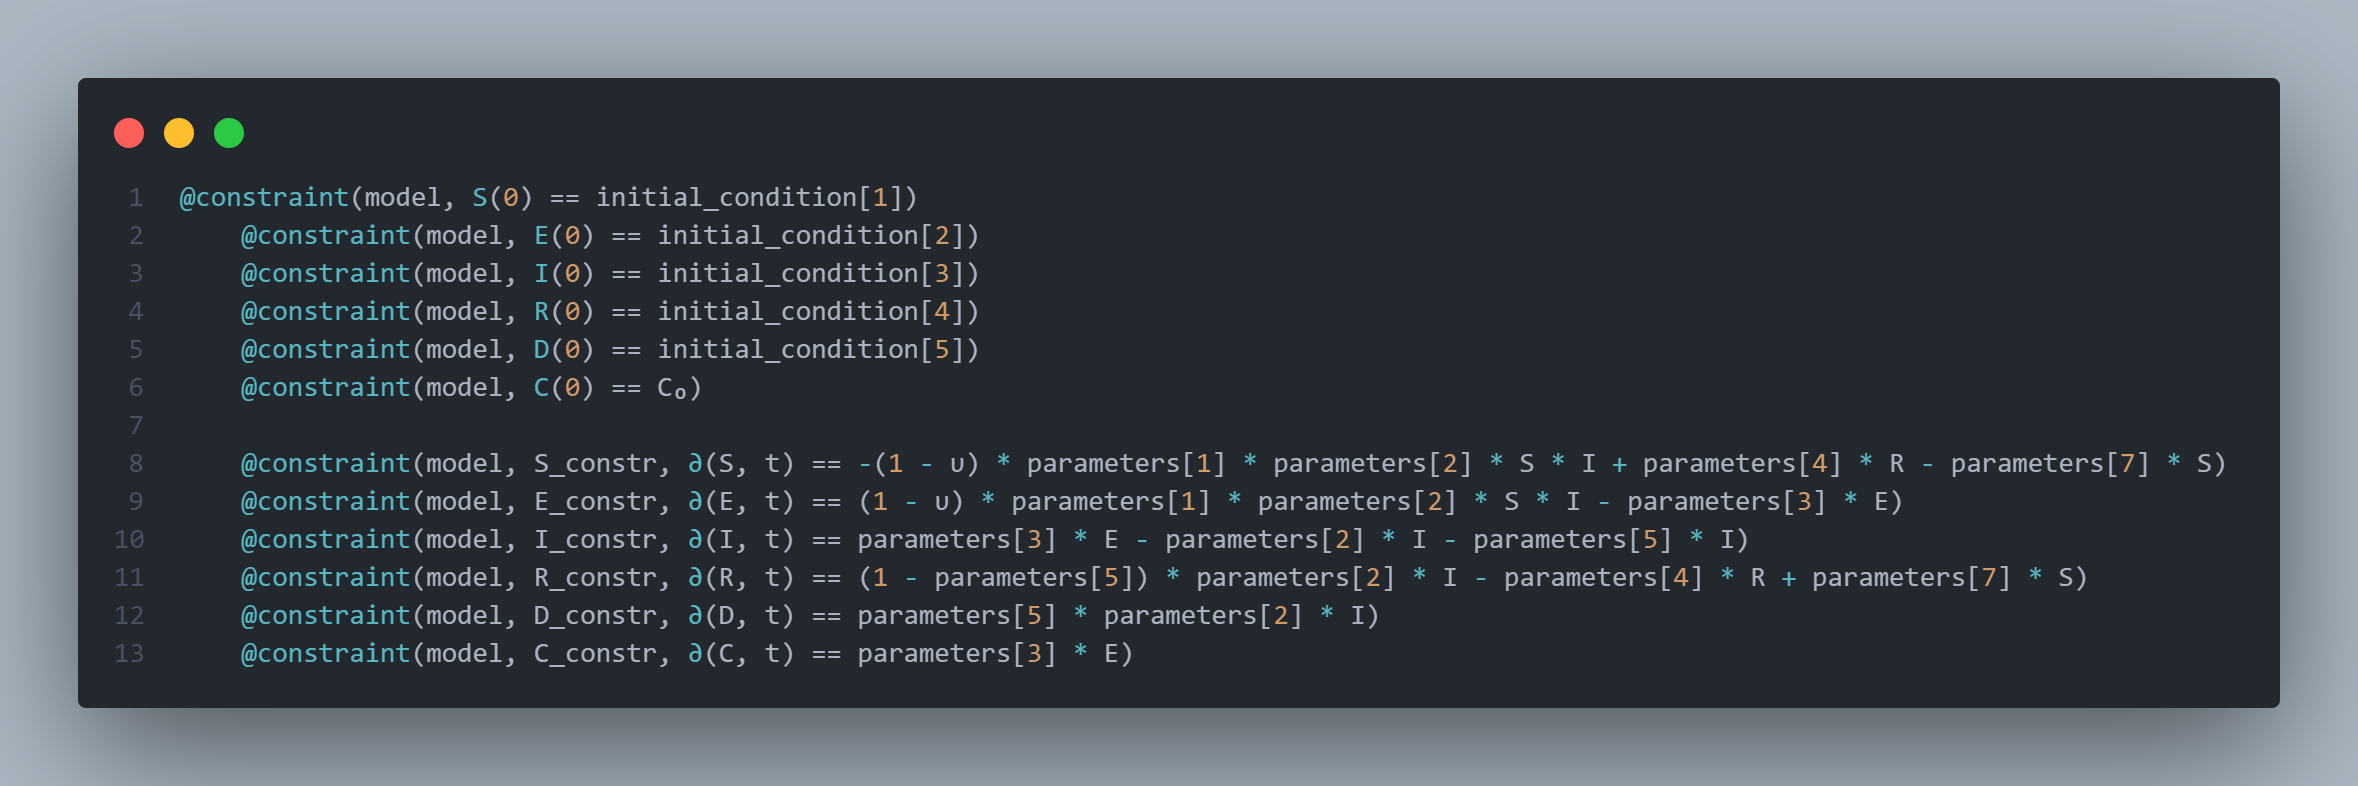
\includegraphics[width=\textwidth]{img/controller_rules.png}
	\captionof{figure}{Definizione regole del modello del controller}
	\label{fig:controller_rules}
\end{minipage}

Essendo che le regole mostrate in figura \ref{fig:controller_rules} sono relative agli stati 
SEIR e l'idea alla base del controllore e' quella di ridurre quanto piu' possibile il numero di
infetti cumulati che ci sono all'interno del sistema, e' stato aggiunto uno stato che descrive
appunto questo stato aggiuntivo.

Successivamente vi sono delle regole su quanto il modello puo' impiegare in termini di risorse, 
le quali sono le nostre contromisure con relativo costo, dato dall'integrale del valore della nostra
contromisura applicata nel tempo.

\begin{minipage}{\linewidth}
	\centering
	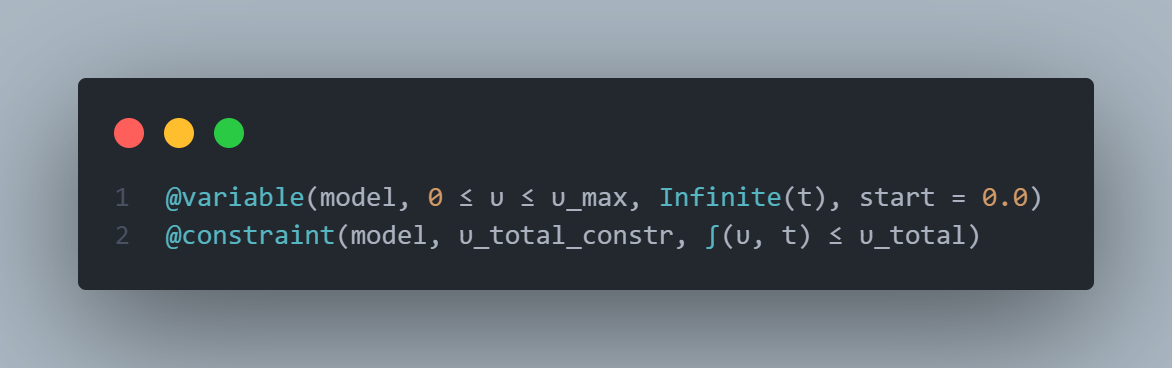
\includegraphics[width=\textwidth]{img/controller_rules_1.png}
	\captionof{figure}{Definizione regole del modello del controller per le contromisure}
	\label{fig:controller_rules_1}
\end{minipage}

Infine viene ottimizzato il modello e ritornato il valore medio delle contromisure applicate
quando applicate. 

\subsubsection{SciML.ai}

L'utilizzo della suite \textbf{SciML.ai} e' stato fatto per l'integrazione
di un modello di Machine Learning in un sistema di monitoraggio e possibilmente di 
intervento. Applicare un algoritmo di ML per predire l'andamento di un sistema non lineare dinamico 
senza avere una grande base di dati puo' risultare problematico e i risultati possono risultare 
poco affidabili. Lo sviluppo di tecniche che congiungono la modellazione puramente matematica
alla flessibilita' delle reti neurali ha permesso di sviluppare approcci \emph{data-driven domain-specific} 
\cite{rackauckas2020universal} \cite{Kim_2021} \cite{dandekar2022bayesian} \cite{chen2019neural}
che permettono di ottenere risultati affidabili pur avendo una base di dati scarsa.

\subsubsection*{Addestramento}

\subsubsection*{Predizione}

\subsubsection*{UDE e Neural Network}

\subsubsection*{Raffinamento con SINDy}

\subsubsection*{Utilizzo GPU}

\subsubsection{Applicabilità al mondo reale}

\subsubsection{Grafici}